\section{Three-seed 50k CIFAR-10 FID}

The paper-scale CIFAR-10 run evaluates the PNDM backend
\citep{liu2022pndm} with \texttt{pndm\_model\_ddim\_cifar10}, Euler solver,
seeds 0, 1, and 2, NFE 10 and 20, and base, native-coordinate linear, fixed
Karras/EDM-style \citep{karras2022edm}, authorized project-owned offline-proxy,
and our schedules. Each seed uses 50k generated images for FID. The table
reports mean and standard error over seeds.

\begin{figure}[t]
  \centering
  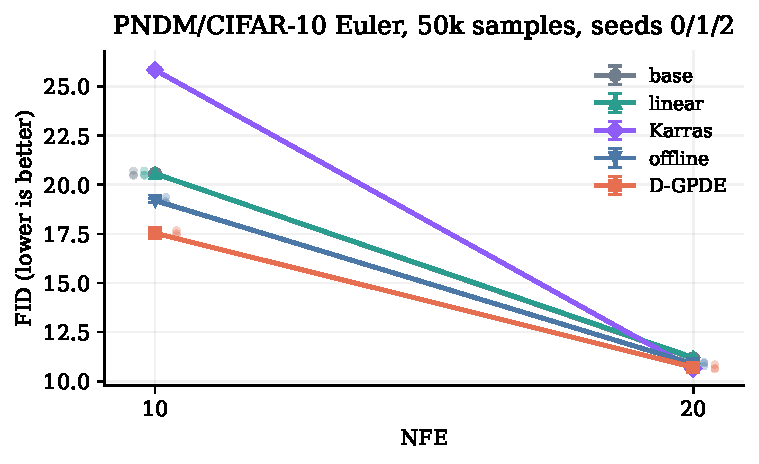
\includegraphics[width=0.68\linewidth]{figures/cifar10_pndm_euler_50k_fid_seeds0_1_2.pdf}
  \caption{PNDM/CIFAR-10 50k FID for model
  \texttt{pndm\_model\_ddim\_cifar10}, Euler solver, base, native-coordinate
  linear, fixed Karras/EDM-style, authorized project-owned offline-proxy, and
  our schedules, NFE 10 and 20, seeds 0, 1, and 2, final generation
  metric FID where lower is better. Error bars show standard error.}
  \label{fig:cifar10-pndm-euler-50k-seeds0-1-2}
\end{figure}

Figure~\ref{fig:cifar10-pndm-euler-schedule-profile-nfe20} shows the NFE-20
schedule profiles for the seed-0 calibration artifact used in the table. The
base and native-linear start grids overlap in this backend. Karras shifts more
steps toward the low-noise end, while ours redistributes start timesteps
toward the regions selected by the defect monitor.

\begin{figure}[t]
  \centering
  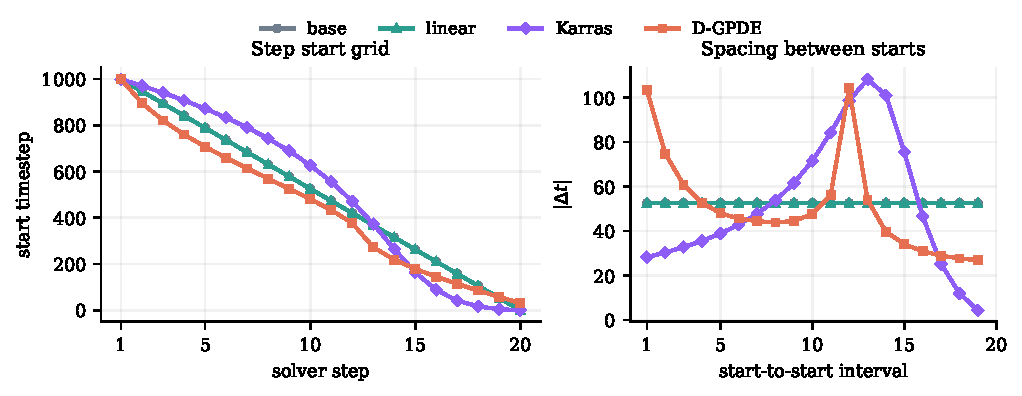
\includegraphics[width=0.78\linewidth]{figures/cifar10_pndm_euler_nfe20_schedule_profile_seed0.pdf}
  \caption{PNDM/CIFAR-10 Euler NFE-20 schedule profile for
  \texttt{pndm\_model\_ddim\_cifar10}, seed 0. The left panel shows solver-step
  start timesteps for base, native-coordinate linear, Karras/EDM-style, and
  our schedules. The right panel shows spacing between consecutive start
  timesteps. This is a schedule diagnostic, not an additional image-quality
  metric.}
  \label{fig:cifar10-pndm-euler-schedule-profile-nfe20}
\end{figure}

\begin{table}[t]
  \centering
  \caption{Actual seed-0 schedule reuse for PNDM/CIFAR-10 with
  \texttt{pndm\_model\_ddim\_cifar10}, Euler solver, NFE 10 and 20,
  seeds 1 and 2, and 50k generated images per seed. FID is
  lower-is-better. The reuse gap is seed-0-reuse FID minus seed-specific
  FID for our schedule. For these rows the continuous schedules differ by
  less than 0.002 timestep units and round to the same integer
  PNDM Euler execution grids.}
  \label{tab:cifar10-pndm-euler-50k-reuse-seed0-schedule}
  \begin{tabular}{rrrrr}
    \toprule
    NFE & base & per-seed ours & reused ours & reuse gap \\
    \midrule
    10 & 20.49 $\pm$ 0.02 & 17.47 $\pm$ 0.05 & 17.47 $\pm$ 0.05 & 0.000 $\pm$ 0.000 \\
    20 & 11.10 $\pm$ 0.02 & 10.64 $\pm$ 0.02 & 10.64 $\pm$ 0.02 & 0.000 $\pm$ 0.000 \\
    \bottomrule
  \end{tabular}
\end{table}


Table~\ref{tab:cifar10-pndm-euler-50k-reuse-seed0-schedule} reports an actual
generation reuse check: the seed-0 schedule bundle was loaded for
seeds 1 and 2, and FID was recomputed from 50k generated images per seed. In
this PNDM Euler backend, the continuous seed-specific schedules differ from the
seed-0 schedule by less than 0.002 timestep units. They round to the same
integer execution timesteps, so the reuse check verifies no execution-level FID
penalty for this configuration. It does not establish transfer across models,
solvers, prompt distributions, or CFG conditions.

The cleaned metric rows, copied schedules, linear and Karras metadata,
authorized offline metric rows, and oracle-reuse cost and reuse-validation
tables are stored under \texttt{paper/results/cifar10\_50k/}. The paper-facing
archive omits authorized offline numeric schedule bundles.
The source output roots are
\texttt{outputs/gpde\_pndm\_cifar10\_50k\_nfe10\_20\_*} and
\texttt{outputs/gpde\_pndm\_cifar10\_50k\_linear\_baseline\_seeds0\_1\_2/}
and
\texttt{outputs/gpde\_pndm\_cifar10\_50k\_karras\_baseline\_seeds0\_1\_2/}
and
\texttt{outputs/gpde\_pndm\_cifar10\_authorized\_offline/};
the actual reuse run lives under
\texttt{outputs/gpde\_pndm\_cifar10\_50k\_reuse\_seed0\_schedule\_seeds1\_2/}.
